\documentclass[titlepage]{article}
\usepackage[12pt]{extsizes} 
\usepackage[T2A]{fontenc}
\usepackage[utf8]{inputenc}
\usepackage[english,russian]{babel}
%\usepackage{pscyr}
\usepackage{hyperref}
\usepackage{setspace}
\usepackage{amsmath,amssymb,amsfonts,amsthm,secdot}
\usepackage[left=30mm, top=20mm, right=30mm, bottom=20mm, nohead, footskip=15mm]{geometry} 
\usepackage[pdftex]{graphicx}
\usepackage[indentfirst]{titlesec}
\usepackage[usenames]{color}
\usepackage{colortbl}
\usepackage{listings}
\usepackage{pdfpages}
\usepackage{secdot}

\def\l{\left}
\def\r{\right}
\def\le{\leqslant}
\def\ge{\geqslant}
\def\part{\partial}

\begin{document} 

\newtheorem{theorem}{Теорема}
\newtheorem{lemma}{Лемма}
\newtheorem{definition}{Определение}
\renewcommand{\proofname}{Доказательство}

\begin{center}
\hfill \break
\hfill \break
\hfill \break
\LARGE Отчёт о выполнении задания по курсу  \\
\LARGE "Практикум на ЭВМ" \\
\hfill \break
\large Г.В. Мигунов \\
\hfill \break
\today \\

\end{center}

\section{Постановка задачи}
Дана система дифференциальных уравнений:
\begin{equation*}
 \begin{cases}
   \frac{\part u_1}{\part t} = a\frac{\part u_1}{\part x} + b\frac{\part u_2}{\part x}
   \\
	\frac{\part u_2}{\part t} = b\frac{\part u_1}{\part x} + c\frac{\part u_2}{\part x}
 \end{cases}
\end{equation*}

с начальными условиями:
\begin{equation*}
 \begin{cases}
 	u_1(0,x) = \varphi_1(x)
   \\
 	u_3(0,x) = \varphi_2(x)	
 \end{cases}
\end{equation*}

и краевыми условиями:
\begin{equation*}
 \begin{cases}
 	u_1(t,0) = u_1(t,1)
   \\
 	u_2(t,0) = u_2(t,1)
 \end{cases}
\end{equation*}

Требуется найти решение системы, определенное в области $x \in [0,1], t \in [0,+\infty]$ и удовлетворяющее начальным и краевым условиям.
Числа $a, b, c$ и функции $\varphi_1, \varphi_2$ заданы.

\section{Преобразование задачи}
Введем вектор-функции $u = \l(\begin{matrix} u_1 \\ u_2 \end{matrix}\r)$ и $\varphi = \l(\begin{matrix} \varphi_1 \\ \varphi_2 \end{matrix}\r)$ и матрицу $A = \l(\begin{matrix}a & b\\ b & c\end{matrix}\r)$. Тогда исходную задачу можно переписать в следующем виде:
\begin{equation*}
 \begin{cases}
 	\frac{\part u}{\part t} = A\frac{\part u}{\part x}
 	\\
	u(0,x) = \varphi(x)
	\\	
	u(t, 0) = u(t, 1)
 \end{cases}
\end{equation*}

Заметим, что матрица $A$ --- симметрическая, следовательно, она имеет вещественные собственные значения. Пусть $\lambda_1, \lambda_2$ --- эти самые собственные значения, а $\xi_1$ и $\xi_2$ --- соответствующие им собственные вектора.

Пусть $C = \l(\xi_1, \xi_2\r)$ --- матрица, по столбцам которой записаны собственные вектора $\xi_1$ и $\xi_2$ матрицы $A$. Тогда следующим преобразованием мы можем привести матрицу $A$ к диагональному виду: $D = C^{-1}AC = \l(\begin{matrix} \lambda_1 & 0 \\ 0 & \lambda_2 \end{matrix}\r)$.

Произведем следующую замену: $u = Cv$. Тогда:
\begin{gather*}
	C\frac{\part v}{\part t} = AC\frac{\part v}{\part x} 
	\\
	\frac{\part v}{\part t} = C^{-1}AC\frac{\part v}{\part x}
	\\
	\frac{\part v}{\part t} = D\frac{\part v}{\part x}	
\end{gather*}

Таким образом, получим новую задачу:
\begin{equation*}
 \begin{cases}
 	\frac{\part v}{\part t} = D\frac{\part v}{\part x}
 	\\
	v(0, x) = \psi(x)
	\\	
	v(t, 0) = v(t, 1)
 \end{cases}
\end{equation*}

где $\psi(x) = C^{-1}\varphi(x) = \l(\begin{matrix} \psi_1 \\ \psi_2 \end{matrix}\r)$

В силу диагональности матрицы $D$ данная двумерная задача разбивается на две одномерные задачи вида:
\begin{equation*}
 \begin{cases}
 	\frac{\part \omega}{\part t} = \lambda\frac{\part \omega}{\part x}
 	\\
	\omega(0, x) = \nu(x)
	\\	
	\omega(t, 0) = \omega(t, 1)
 \end{cases}
\end{equation*}

Всюду далее мы будем рассматривать задачи именно такого вида.

\section{Построение разностных схем}
Для задачи 
\begin{equation*}
 \begin{cases}
 	\frac{\part \omega}{\part t} = \lambda\frac{\part \omega}{\part x}
 	\\
	\omega(0, x) = \nu(x)
	\\	
	\omega(t, 0) = \omega(t, 1)
 \end{cases}
\end{equation*}
требуется построить три разностные схемы:
\begin{enumerate}
	\item условно устойчивую
	\item безусловно устойчивую
	\item безусловно неустойчивую
\end{enumerate}

Будем исследовать решение задачи в ограниченной области $x \in [0,1], t \in [0, T]$. Для этого построим сетку: зафиксируем натуральные числа $N,M$ и разобьем отрезки $[0,T]$ и $[0,1]$ на $N$ и $M$ равных отрезков соответственно. Длина шага по оси $Ot$ будет равна $\tau := \frac{T}{N}$, а по оси $Ox$ --- $h := \frac{1}{M}$. 

Точки получившейся сетки будут иметь координаты: $(t_n, x_m) = (\tau n, hm), \ n = \overline{0,N}, m = \overline{0,M}$. Таким образом, любая точка сетки задается своими координатами $n$ и $m$. Значение решения задачи в точке с координатами $(n,m)$ будем обозначать $\omega^n_m$.

\begin{figure}[h]
\center
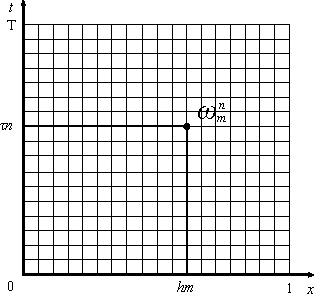
\includegraphics[width = 60mm]{img1.pdf}
\caption{Решение задачи $\omega^n_m$ в точке, заданной координатами $n$ и $m$}
\end{figure}


Для построения разностной схемы мы будем пользоваться шеститочечным шаблоном: 

\begin{figure}[h]
\center
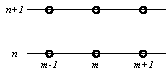
\includegraphics[width = 50mm]{img2.pdf}
\caption{Шеститочечный шаблон}
\end{figure}

\subsection{Условно устойчивая схема}
Для построения условно устойчивой разностной схемы будем использовать значения функции в следующих точках шаблона: 


\begin{figure}
\centering
\begin{minipage}{.5\textwidth}
  \centering
  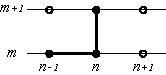
\includegraphics[width = 40mm]{img3.pdf}
  \caption{Схема «Левый треугольник»}
  \label{fig:test1}
\end{minipage}%
\begin{minipage}{.5\textwidth}
  \centering
  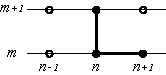
\includegraphics[width = 40mm]{img4.pdf}
  \caption{Схема «Правый треугольник»}
\end{minipage}
\end{figure}

\break

Причем тем или иным способом мы будем пользоваться в зависимости от знака $\lambda$ (см. п. 5).
В первом случае (рис. 3) мы имеем:
\begin{gather*}
	\frac{\part v}{\part t} \to \frac{\omega_m^{n+1} - \omega_m^n}{\tau}
	\\
	\frac{\part v}{\part x} \to \frac{\omega_m^n - \omega_{m-1}^n}{h}
\end{gather*}
Получим схему:
\begin{equation}
 \tag{A}
 \begin{cases}
 	\frac{\omega_m^{n+1} - \omega_m^n}{\tau} = \lambda\frac{\omega_m^n - \omega_{m-1}^n}{h}
 	\\
	\omega_m^0 = \nu(x_n)
	\\	
	\omega_0^n = \omega_M^n
 \end{cases}
\end{equation}

Аналогично, во втором случае (рис. 4):
\begin{equation}
 \tag{B}
 \begin{cases}
 	\frac{\omega_m^{n+1} - \omega_m^n}{\tau} = \lambda\frac{\omega_{m+1}^n - \omega_{m}^n}{h}
 	\\
	\omega_m^0 = \nu(x_n)
	\\	
	\omega_0^n = \omega_M^n
 \end{cases}
\end{equation}

В обоих случаях значение $\omega_m^{n+1}$ в точке с $n+1$ - ого слоя выражается через значения в точках с предыдущих слоёв, а так как слой $\omega_m^0$ нам известен из условия задачи, то таким образом мы найдем значения во всех точках сетки. 

\subsection{Безусловно устойчивая схема}
Для построения безусловно устойчивой разностной схемы будем использовать значения функции в следующих точках шаблона: 
\begin{figure}[h]
\center
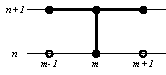
\includegraphics[width = 40mm]{img5.pdf}
\caption{«T» - схема}
\end{figure}

Получим следующую схему:
\begin{equation}
 \tag{C}
 \begin{cases}
 	\frac{\omega_m^{n+1} - \omega_m^n}{\tau} = \lambda\frac{\omega_{m+1}^{n+1} - \omega_{m-1}^{n+1}}{h}
 	\\
	\omega_m^0 = \nu(x_n)
	\\	
	\omega_0^n = \omega_M^n
 \end{cases}
\end{equation}

\section{Порядок аппроксимации}
\subsection{Схема «Левый треугольник»}
Рассмотрим оператор $L_{\tau,h}$:
\begin{equation*}
	L_{\tau,h}{\omega} |_{m,n} := \frac{\omega_m^{n+1} - \omega_m^n}{\tau} - \lambda\frac{\omega_m^n - \omega_{m-1}^n}{h}
\end{equation*}
Порядок аппроксимации найдем, подставив в оператор $L_{\tau,h}$ точное решение задачи и оценив получившееся. Точное решение задачи в точке с координатами $(n,m)$ будем обозначать $\omega(n,m)$.
\begin{equation*}
	L_{\tau,h}{\omega} |_{m,n} = \frac{\omega(n+1,m) - \omega(n,m)}{\tau} - \lambda\frac{\omega(n,m) - \omega(n,m-1)}{h}
\end{equation*}

Разложим функцию $\omega$ в ряд Тейлора в точке $(n,m)$:
\begin{gather*}
	\omega(n+1,m) = \omega(n,m) + \omega'_t(n,m)\tau + \underbar{\textit{O}}(\tau^2) \\
	\omega(n,m-1) = \omega(n,m) - \omega'_x(n,m)h + \underbar{\textit{O}}(h^2)
\end{gather*}

Тогда, так как $\omega'_t(n,m) - \lambda\omega'_x(n,m) = 0$ (поскольку $\omega(n,m)$ --- точное решение задачи), получим:
\begin{multline*}
	L_{\tau,h}{\omega} |_{m,n} = \frac{\omega(n,m) + \omega'_t(n,m)\tau + \underbar{\textit{O}}(\tau^2) - \omega(n,m)}{\tau} - \\ 
	 - \lambda\frac{\omega(n,m) - (\omega(n,m) - \omega'_x(n,m)h + \underbar{\textit{O}}(h^2))}{h} = \\
	 = \omega'_t(n,m) + \underbar{\textit{O}}(\tau) - \lambda\omega'_x(n,m) + \underbar{\textit{O}}(h) = \underbar{\textit{O}}(\tau + h)
\end{multline*}

\subsection{Схема «Правый треугольник»}
Так же, как и с предыдущей схемой, произведем аналогичные преобразования:
\begin{equation*}
	L_{\tau,h}{\omega} |_{m,n} = \frac{\omega(n+1,m) - \omega(n,m)}{\tau} - \lambda\frac{\omega(n,m+1) - \omega(n,m)}{h}
\end{equation*}

Разложим функцию $\omega$ в ряд Тейлора в точке $(n,m)$:
\begin{gather*}
	\omega(n+1,m) = \omega(n,m) + \omega'_t(n,m)\tau + \underbar{\textit{O}}(\tau^2) \\
	\omega(n,m+1) = \omega(n,m) + \omega'_x(n,m)h + \underbar{\textit{O}}(h^2)
\end{gather*}
\begin{multline*}
	L_{\tau,h}{\omega} |_{m,n} = \frac{\omega(n,m) + \omega'_t(n,m)\tau + \underbar{\textit{O}}(\tau^2) - \omega(n,m)}{\tau} - \\ 
	 - \lambda\frac{\omega(n,m) + \omega'_x(n,m)h + \underbar{\textit{O}}(h^2) -\omega(n,m)}{h} = \\
	 = \omega'_t(n,m) + \underbar{\textit{O}}(\tau) - \lambda\omega'_x(n,m) + \underbar{\textit{O}}(h) = \underbar{\textit{O}}(\tau + h)
\end{multline*}

\subsection{Схема «T»}
\begin{equation*}
	L_{\tau,h}{\omega} |_{m,n} = \frac{\omega(n+1,m) - \omega(n,m)}{\tau} - \lambda\frac{\omega(n+1,m+1) - \omega(n+1,m-1)}{h}
\end{equation*}

Разложим функцию $\omega$ в ряд Тейлора в точке $(n+1,m)$:
\begin{gather*}
	\omega(n,m) = \omega(n+1,m) - \omega'_t(n+1,m)\tau + \underbar{\textit{O}}(\tau^2) \\
	\omega(n+1,m+1) = \omega(n+1,m) + \omega'_x(n+1,m)h + \omega''_{xx}(n+1,m)h^2 + \underbar{\textit{O}}(h^3) \\
	\omega(n+1,m-1) = \omega(n+1,m) - \omega'_x(n+1,m)h + \omega''_{xx}(n+1,m)h^2 + \underbar{\textit{O}}(h^3)
\end{gather*}
Подставим получившиеся разложения в оператор $L_{\tau,h}{\omega} |_{m,n}$
\begin{multline*}
	L_{\tau,h}{\omega} |_{m,n} = \frac{\omega(n+1,m) - (\omega(n,m) = \omega(n+1,m) - \omega'_t(n+1,m)\tau + \underbar{\textit{O}}(\tau^2))}{\tau} - \\
	- \lambda \biggl[ \frac{\omega(n+1,m) + \omega'_x(n+1,m)h + \omega''_{xx}(n+1,m)h^2 + \underbar{\textit{O}}(h^3)}{2h} - \\
	- \frac{\omega(n+1,m) - \omega'_x(n+1,m)h + \omega''_{xx}(n+1,m)h^2 + \underbar{\textit{O}}(h^3)}{2h} \biggr] = \\
	= \omega'_t(n+1,m) + \underbar{\textit{O}}(\tau) - \lambda\omega'_x(n+1,m) + \underbar{\textit{O}}(h^2) = \underbar{\textit{O}}(\tau + h^2)
\end{multline*}

Для определения порядка аппроксимации воспользуемся следующей нормой:
\begin{equation*}
	\|u\| = h\tau\sum_{m=0}^{M}\sum_{n=0}^{N}{|u_{m,n}|}
\end{equation*}

Аппроксимация исходной задачи схемами (A), (B) и (C) имеет место в том случае, когда 
\begin{equation*}
	\|A_{h,\tau}[\omega]_{h,\tau} - F_{h,\tau}\| \to 0, \quad h,\tau \to 0
\end{equation*}
где:
\begin{enumerate}
	\item $A_{h,\tau}$ -- матрица системы линейных уравнений, соответствующей разностной схеме (A), (B) или (C)
	\item $F_{h,\tau}$ -- свободный столбец той же системы линейных уравнений
	\item $[\omega]_{h,\tau}$ -- точное решение исходной задачи, взятое в узлах сетки
\end{enumerate}

Для схемы «Левый треугольник» имеем:
$$F_{h,\tau} = 0$$
\begin{multline*}
	\|A_{h,\tau}[\omega]_{h,\tau} - F_{h,\tau}\| = h\tau\sum_{m=0}^{M}\sum_{n=0}^{N}{|L_{h,\tau}\omega|_{m,n}|} \le \\
	\le h\tau\sum_{m=0}^{M}\sum_{n=0}^{N}{C_{n,m}\cdot(\tau+h)} \le \\
	\le \frac{T}{N}\frac{1}{M} \cdot NM \cdot \max_{n,m}{C_{n,m}} \cdot (\tau+h) = C \cdot (\tau+h)
\end{multline*}

Таким образом, аппроксимация схемы «Левый треугольник» установлена. Аналогичными рассуждениями устанавливается аппроксимация схемы «Правый треугольник».

Для схемы «Т» имеем:
$$F_{h,\tau} = 0$$
\begin{multline*}
	\|A_{h,\tau}[\omega]_{h,\tau} - F_{h,\tau}\| = h\tau\sum_{m=0}^{M}\sum_{n=0}^{N}{|L_{h,\tau}\omega|_{m,n}|} \le \\
	\le h\tau\sum_{m=0}^{M}\sum_{n=0}^{N}{C_{n,m}\cdot(\tau+h^2)} \le \\
	\le \frac{T}{N}\frac{1}{M} \cdot NM \cdot \max_{n,m}{C_{n,m}} \cdot (\tau+h^2) = C \cdot (\tau+h^2)
\end{multline*}

\section{Исследование устойчивости}
Для того, чтобы установить устойчивость или неустойчивость схемы, будем пользоваться спектральным признаком устойчивости (СПУ). 
Пусть на сетке с узлами $(n,m)$ построена разностная схема
$$L_{h,\tau}\omega_{h,\tau}|_{n,m} = 0$$
Если любое частное решение уравнения $L_{h,\tau}\omega_{h,\tau}|_{n,m} = 0$, имеющее вид 
$$\omega_m^n = \mu^ne^{im\varphi}$$ 
для любых $\varphi$ равномерно ограничено по $n$, то схема является устойчивой. В противном случае, схема устойчивой не является.

\subsection{Схема «Левый треугольник»}
Запишем разностную схему для данного случая:
\begin{equation*}
	L_{\tau,h}{\omega} |_{m,n} := \frac{\omega_m^{n+1} - \omega_m^n}{\tau} - \lambda\frac{\omega_m^n - \omega_{m-1}^n}{h} = 0
\end{equation*}
Подставим $\omega(n,m) = \omega_m^n = \mu^ne^{im\alpha}$ и выясним, при каких $\mu$ эта функция будет являться решением:
\begin{equation*}
	\frac{\mu^{n+1}e^{im\alpha} - \mu^ne^{im\alpha}}{\tau} = \lambda\frac{\mu^ne^{im\alpha} - \mu^ne^{i(m-1)\alpha}}{h}
\end{equation*}
Сократим на $\mu^ne^{im\alpha}$ и преобразуем получившееся равенство:
\begin{gather*}
	\frac{\mu-1}{\tau} = \lambda\frac{1-e^{-i\alpha}}{h} \\
	\mu = 1 + r - re^{-i\alpha}
\end{gather*}
где $r = \frac{\lambda\tau}{h}$.

Очевидно, данная функция равномерно ограничена по $n$, так как $|\mu| \le 1 \ \forall \alpha$.
Множество значений $\mu$ -- окружность $Q$ на комплексной плоскости с центром в точке $1+r$ и радиуса $r$. Она касается единичной окружности в точке $1$. Поэтому, если $r > 0$, то вся окружность $Q$ лежит вне единичного круга, следовательно, схема неустойчива. В случае, если $|r < 0|$, схема будет устойчива, если $|r| \ge -1$ и неустойчива в остальных случаях. 
\hfill \break
\hfill \break
\hfill \break

\textbf{Вывод:} 
\begin{enumerate}
	\item Если $\lambda > 0$, то $r = \frac{\lambda\tau}{h} > 0$ и схема безусловно неустойчива
	\item Если $\lambda < 0$, то $r = \frac{\lambda\tau}{h} < 0$. Схема устойчива при $\lambda \ge -\frac{h}{\tau}$ и неустойчива в остальных случаях. Получили условно устойчивую схему.
\end{enumerate}

\subsection{Схема «Правый треугольник»}
Приведем аналогичные рассуждения. Запишем разностную схему:
\begin{equation*}
	L_{\tau,h}{\omega} |_{m,n} := \frac{\omega_m^{n+1} - \omega_m^n}{\tau} - \lambda\frac{\omega_{m+1}^n - \omega_m^n}{h} = 0
\end{equation*}
Подставим $\omega(n,m) = \omega_m^n = \mu^ne^{im\alpha}$ и выясним, при каких $\mu$ эта функция будет являться решением:
\begin{equation*}
	\frac{\mu^{n+1}e^{im\alpha} - \mu^ne^{im\alpha}}{\tau} = \lambda\frac{\mu^ne^{i(m+1)\alpha} - \mu^ne^{im\alpha}}{h}
\end{equation*}
Сократим на $\mu^ne^{im\alpha}$ и преобразуем получившееся равенство:
\begin{gather*}
	\frac{\mu-1}{\tau} = \lambda\frac{e^{i\alpha} - 1}{h} \\
	\mu = 1 - r + re^{i\alpha}
\end{gather*}
где $r = \frac{\lambda\tau}{h}$.

Очевидно, данная функция равномерно ограничена по $n$, так как $|\mu| \le 1 \ \forall \alpha$.
Множество значений $\mu$ -- окружность $Q$ на комплексной плоскости с центром в точке $1-r$ и радиуса $r$. Она касается единичной окружности в точке $1$. Поэтому, если $r < 0$, то вся окружность $Q$ лежит вне единичного круга, следовательно, схема неустойчива. В случае, если $|r > 0|$, схема будет устойчива, если $|r| \le 1$ и неустойчива в остальных случаях. 
\hfill \break

\textbf{Вывод:} 
\begin{enumerate}
	\item Если $\lambda < 0$, то $r = \frac{\lambda\tau}{h} < 0$ и схема безусловно неустойчива
	\item Если $\lambda > 0$, то $r = \frac{\lambda\tau}{h} > 0$. Схема устойчива при $\lambda \le \frac{h}{\tau}$ и неустойчива в остальных случаях. Получили условно устойчивую схему.
\end{enumerate}
\hfill \break

\textbf{В итоге} при  $\lambda < 0$ в качестве условно устойчивой разностной схемы выбираем схему «Левый треугольник», а в качестве безусловно неустойчивой - «Правый треугольник». При  $\lambda > 0$ в качестве условно устойчивой разностной схемы выбираем схему «Правый треугольник», а в качестве безусловно неустойчивой - «Левый треугольник».

\subsection{Схема «T»}
\begin{equation*}
	L_{\tau,h}{\omega} |_{m,n} := \frac{\omega_m^{n+1} - \omega_m^n}{\tau} - \lambda\frac{\omega_{m+1}^{n+1} - \omega_{m-1}^{n+1}}{2h} = 0
\end{equation*}
Подставим $\omega(n,m) = \omega_m^n = \mu^ne^{im\alpha}$:
\begin{equation*}
	\frac{\mu^{n+1}e^{im\alpha} - \mu^ne^{im\alpha}}{\tau} - \lambda\frac{\mu^{n+1}e^{i(m+1)\alpha} - \mu^{n+1}e^{i(m-1)\alpha}}{2h} = 0
\end{equation*}
Сократим на $\mu^ne^{im\alpha}$ и преобразуем получившееся равенство:
\begin{gather*}
	\frac{\mu-1}{\tau} - \frac{\mu \lambda i}{h}\frac{e^{i\alpha} - e^{-i\alpha}}{2i} = 0 \\
	\frac{\mu - 1}{\tau} - \frac{\mu \lambda i}{h}\sin{\alpha} = 0 \\
	\mu = 1 + r \mu i \sin{\alpha},
\end{gather*}
где $r = \frac{\lambda \tau}{h}$


\begin{gather*}
	\mu = \frac{1}{1 - ri\sin{\alpha}} \\
	|\mu| = \l|\frac{1}{1 - ri\sin{\alpha}}\r| = \l|\frac{1 + ri\sin{\alpha}}{1 - r^2\sin^2{\alpha}}\r| = 1
\end{gather*}

Условие $|\mu| = 1 \le 1$ выполнено $\forall \alpha$, следовательно данная схема является безусловно устойчивой.

\section{Циклическая прогонка}
Рассмотрим систему уравнений:

\begin{equation*}
	\begin{cases}
		a_1y_N - c_1y_1 + b_1y_2 = f_1 \\
		a_iy_{i-1} - c_iy_i + b_iy_{i+1} = f_i \quad i = 2,3,\dots,N-1 \\
		a_Ny_{N-1} - c_Ny_N + b_Ny_1 = f_N
	\end{cases}
\end{equation*}

Требуется найти периодическое $(y_{i+N} = y_i)$ решение системы уравнений при следующих условиях:

\begin{equation*}
	a_{i+N} = a_i, \quad b_{i+N} = b_i, \quad c_{i+N} = c_i, \quad f_{i+N} = f_i
\end{equation*}

Будем предполагать, что условие $|c_i| > |a_i| + |b_i|$ (условие диагонального преобладания) выполняется.

Перепишем систему в векторном виде: 
\begin{equation*}
	A_N \vec y_N = \vec f_N, \quad \text{где}
\end{equation*}

\begin{equation*}
	\vec y_N = \l(\begin{matrix} y_1 \\ \vdots \\ y_N \end{matrix}\r), \quad \vec f_N = \l(\begin{matrix} f_1 \\ \vdots \\ f_N \end{matrix}\r) 
\end{equation*}

\begin{equation*}
	A_N = \begin{pmatrix}
		-c_1 & b_1 & 0 & 0 & \dots & 0 & 0 & a_1 \\
		a_2 & -c_2 & b_2 & 0 & \dots & 0 & 0 & 0 \\
		0 & a_3 & -c_3 & b_3 & \dots & 0 & 0 & 0 \\
		\dots & \dots & \dots & \dots & \dots & \dots & \dots & \dots \\
		0 & 0 & 0 & 0 & \dots & -c_{N-2} & b_{N-2} & 0 \\
		0 & 0 & 0 & 0 & \dots & a_{N-1} & -c_{N-1} & b_{N-1} \\
		b_N & 0 & 0 & 0 & \dots & 0 & a_N & -c_N \\
	\end{pmatrix}
\end{equation*}

Для решения перепишем векторную запись системы:
\begin{gather*}
	A_{N-1}\vec y_{N-1} + \vec u_{N-1}y_N = \vec f_{N-1} \\
	\vec v_{N-1}^T \vec y_{N-1} - c_Ny_N = f_N, \quad \text{где} \tag{1}
\end{gather*}

\begin{equation*}
	A_{N-1} = \begin{pmatrix}
		-c_1 & b_1 & 0 & 0 & \dots & 0 & 0 \\
		a_2 & -c_2 & b_2 & 0 & \dots & 0 & 0 \\
		0 & a_3 & -c_3 & b_3 & \dots & 0 & 0 \\
		\dots & \dots & \dots & \dots & \dots & \dots & \dots \\
		0 & 0 & 0 & 0 & \dots & -c_{N-2} & b_{N-2} \\
		0 & 0 & 0 & 0 & \dots & a_{N-1} & -c_{N-1} \\
	\end{pmatrix}
\end{equation*}

\begin{equation*}
	\vec u_{N-1} = \l(\begin{matrix} a_1 \\ 0 \\ \vdots \\ 0 \\ b_{N-1} \end{matrix}\r), \quad 
	\vec v_{N-1} = \l(\begin{matrix} b_N \\ 0 \\ \vdots \\ 0 \\ a_{N} \end{matrix}\r), \quad
	\vec y_{N-1} = \l(\begin{matrix} y_1 \\ y_2 \\ \vdots \\ y_{N-2} \\ y_{N-1} \end{matrix}\r), \quad
	\vec f_{N-1} = \l(\begin{matrix} f_1 \\ f_2 \\ \vdots \\ f_{N-2} \\ f_{N-1} \end{matrix}\r)
\end{equation*}

Решение уравнения $\vec v_{N-1}^T \vec y_{N-1} - c_Ny_N = f_N$ представим в виде:
\begin{equation*}
	\vec y_{N-1} = \vec p_{N-1} = y_N \vec q_{N-1}, \tag{2}
\end{equation*}
где $\vec p_{N-1}$ и $\vec q_{N-1}$ --- решения задач:
\begin{equation*}
	A_{N-1}\vec p_{N-1} = \vec f_{N-1}, \quad A_{N-1}\vec q_{N-1} = -\vec u_{N-1}, \tag{3}
\end{equation*}

решения которых находятся методом обычной прогонки. 

Таким образом, из предыдущих формул получаем:
\begin{equation*}
	y_N = \frac{-f_N + \vec v_{N-1}^T\vec p_{N-1}}{c_N - \vec v_{N-1}^T\vec q_{N-1}}
\end{equation*}

$\vec y_{N-1}$ находим из (2).

Метод циклической прогонки является устойчивым, так как решения (3) находятся с использованием метода прогонки, который, в нашем предположении о преобладании диагональных элементов, является устойчивым.

\subsection{Реализация циклической прогонки}
Методом циклической прогонки нам будет необходимо воспользоваться только в случае схемы «Т». По условию $\omega_0^n = \omega_m^n$ мы можем продолжить решение задачи периодически из области $x \in [0,1], T \in [0,T]$ в полосу $x \in [-\infty, \infty], T \in [0,T]$. Периодичность запишется следующим образом: $\omega_m^n = \omega_{m+M}^n$.

Значения в $m+1$ -- слое выражаются через значения в $m$ -- слое следующим образом:
\begin{gather*}
	\frac{\omega_m^{n+1} - \omega_m^n}{\tau} - \lambda\frac{\omega_{m+1}^{n+1} - \omega_{m-1}^{n+1}}{2h} = 0 \\
	\omega_m^{n+1} - \frac{r}{2}\omega_{m+1}^{n+1} + \frac{r}{2}\omega_{m-1}^{n+1} = \omega_m^n \\
	-\frac{r}{2}\omega_{m-1}^{n+1} - \omega_m^{n+1} + \frac{r}{2}\omega_{m+1}^{n+1} = -\omega_m^n, 
\end{gather*}
где $r = \frac{\lambda\tau}{h}$.
На $n$-ом шаге $n=0,1,\dots,N-1$ значения $\omega_m^n$ нам известны. Получим следующую систему уравнений:

\begin{equation*}
	\begin{cases}
		a_0y_{M-1} - c_0y_0 + b_0y_1 = f_0 \\
		a_iy_{i-1} - c_iy_i + b_iy_{i+1} = f_i \quad i = 2,3,\dots,M-2 \\
		a_{M-1}y_{M-2} - c_{M-1}y_{M-1} + b_{M-1}y_0 = f_{M-1}
	\end{cases}
\end{equation*}

где

\begin{gather*}
	y_i = \omega_{i}^{n+1}, \quad i = 0, 1, \dots, M-1, \\
	f_i = -\omega_{i}^{n}, \quad i = 0, 1, \dots, M-1, \\ 
	a_i = -\frac{r}{2}, \quad c_i = 1, \quad b_i = \frac{r}{2} \quad i = 0, 1, \dots, M-1,
\end{gather*}

В векторной записи: 
\begin{equation*}
	A_n \vec y_n = \vec f_n,
\end{equation*}

\begin{equation*}
	\vec y_n = \l(\begin{matrix} y_0 \\ y_1 \\ \vdots \\ y_{M-1} \end{matrix}\r), \quad \vec f_n = -\l(\begin{matrix} \omega_0^n \\ \omega_1^n \\ \vdots \\ \omega_{M-1}^n \end{matrix}\r) 
\end{equation*}

\begin{equation*}
	A_N = \begin{pmatrix}
		-1 & \frac{r}{2} & 0 & 0 & \dots & 0 & 0 & -\frac{r}{2} \\
		-\frac{r}{2} & -1 & \frac{r}{2} & 0 & \dots & 0 & 0 & 0 \\
		0 & -\frac{r}{2} & -1 & \frac{r}{2} & \dots & 0 & 0 & 0 \\
		\dots & \dots & \dots & \dots & \dots & \dots & \dots & \dots \\
		0 & 0 & 0 & 0 & \dots & -1 & \frac{r}{2} & 0 \\
		0 & 0 & 0 & 0 & \dots & -\frac{r}{2} & -1 & \frac{r}{2} \\
		\frac{r}{2} & 0 & 0 & 0 & \dots & 0 & -\frac{r}{2} & -1 \\
	\end{pmatrix}
\end{equation*}

Решаем систему методом циклической прогонки, переходим к поиску значений на следующем слое. Сходимость метода прогонки может нарушаться при произвольном выборе параметров $\tau$ и $h$. Необходимо так их подобрать, чтобы выполнялось неравенство:
\begin{gather*}
	1 = |c_i| > |a_i| + |b_i| = \frac{r}{2} + \frac{r}{2} = r \\
	\frac{\lambda\tau}{h} = r < 1
\end{gather*}

\section{Начальные условия}
\indent \textbf{1. }
	$$\varphi_1(x) = \sin{2 \pi x}, \qquad \varphi_2(x) = \cos{2 \pi x}$$
\indent \textbf{2. }
	$$\varphi_1(x) = \sin{2 \pi x}, \qquad \varphi_2(x) = \sin{2 \pi x} + \frac{1}{10}\sin{100 \pi x}$$
\indent \textbf{3. }
	$$\varphi_1(x) = x(1-x), \qquad 
	\begin{cases}
		x, & x \in \l[0, \frac{1}{4}\r] \\
		-2\l(x-\frac{1}{2}\r)^2 + \frac{3}{8}, & x \in \l[\frac{1}{4}, \frac{3}{4}\r] \\
		1-x, & x \in \l[\frac{3}{4}, 1\r]
	\end{cases}$$
\newpage

\section{Результаты счёта}

\begin{figure}[h]
\centering
\begin{minipage}{.5\textwidth}
  \centering
  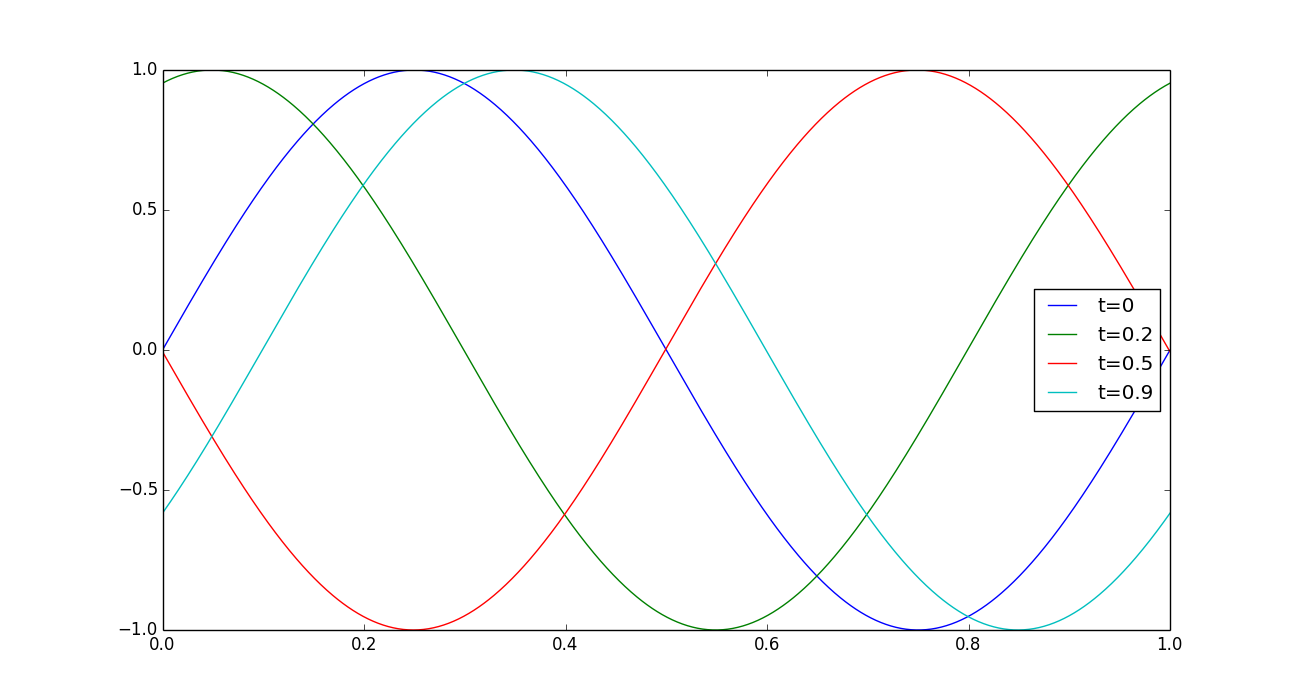
\includegraphics[width = \textwidth]{1_1.png}
  \caption{$u_1(t,x)$, начальные условия №1}
  \label{fig:test1}
\end{minipage}%
\begin{minipage}{.5\textwidth}
  \centering
  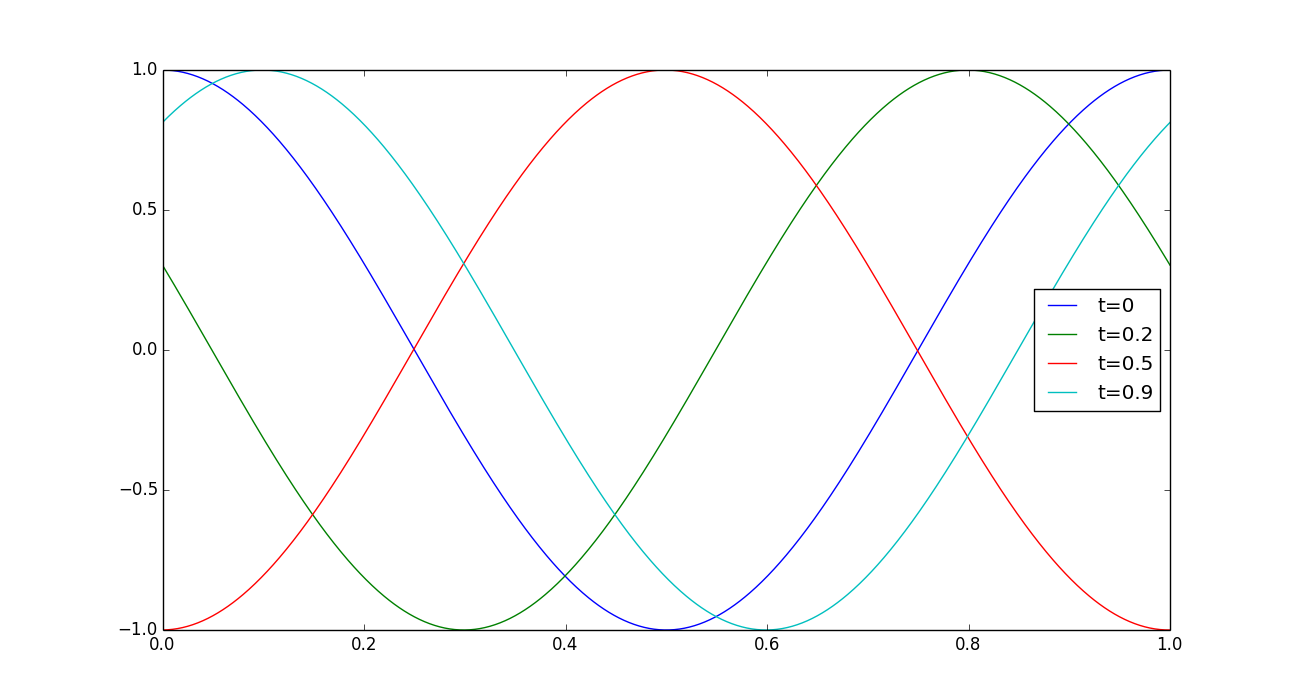
\includegraphics[width = \textwidth]{1_2.png}
  \caption{$u_2(t,x)$, начальные условия №1}
\end{minipage}

\begin{minipage}{.5\textwidth}
  \centering
  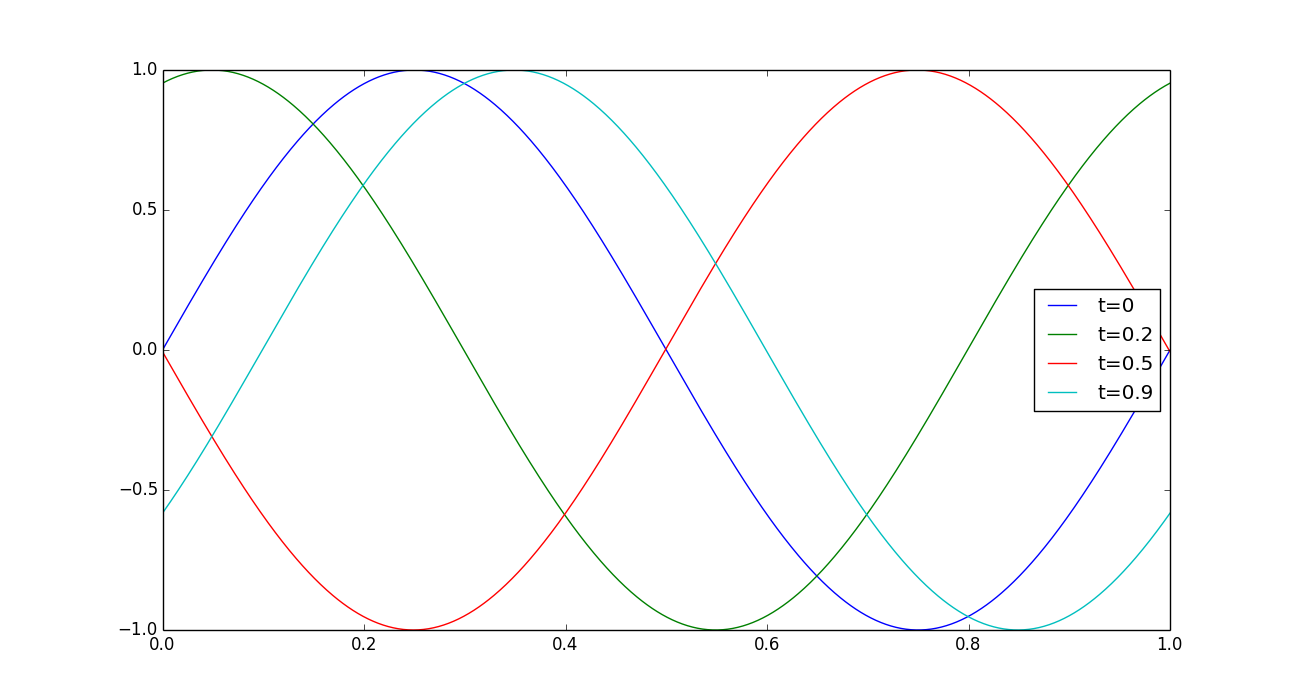
\includegraphics[width = \textwidth]{2_1.png}
  \caption{$u_1(t,x)$, начальные условия №2}
  \label{fig:test1}
\end{minipage}%
\begin{minipage}{.5\textwidth}
  \centering
  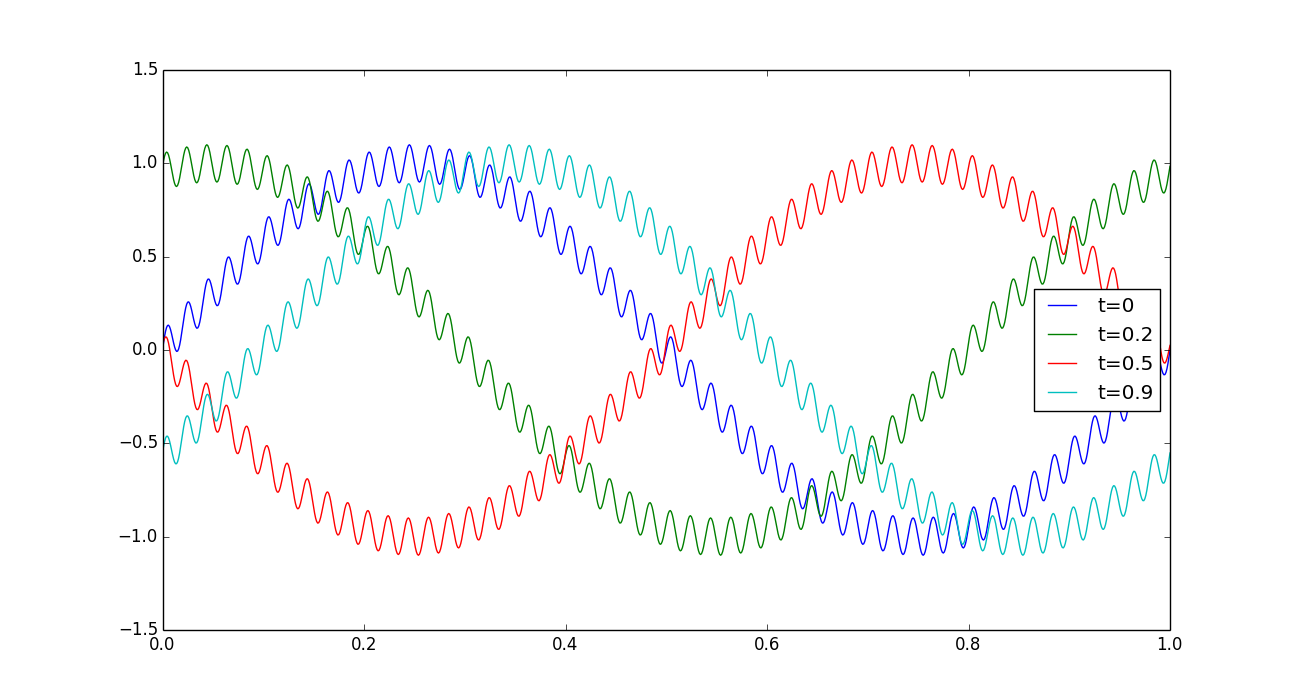
\includegraphics[width = \textwidth]{2_2.png}
  \caption{$u_2(t,x)$, начальные условия №2}
\end{minipage}

\begin{minipage}{.5\textwidth}
  \centering
  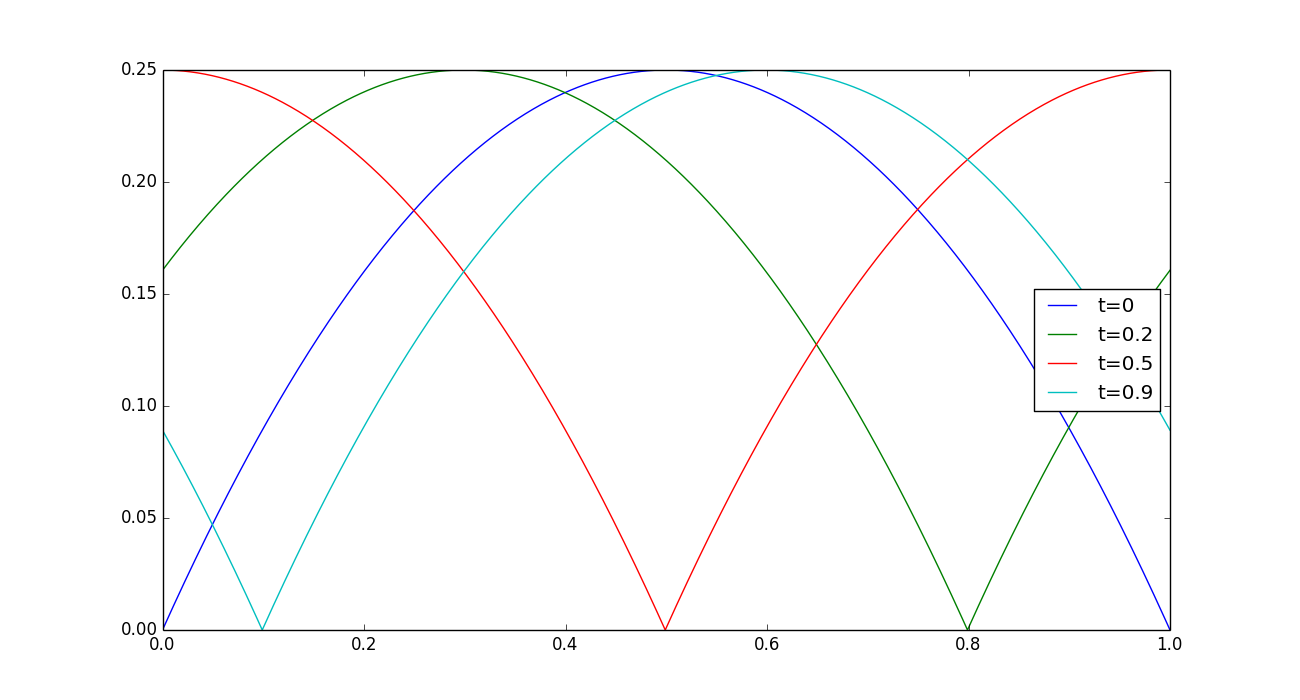
\includegraphics[width = \textwidth]{3_1.png}
  \caption{$u_1(t,x)$, начальные условия №3}
  \label{fig:test1}
\end{minipage}%
\begin{minipage}{.5\textwidth}
  \centering
  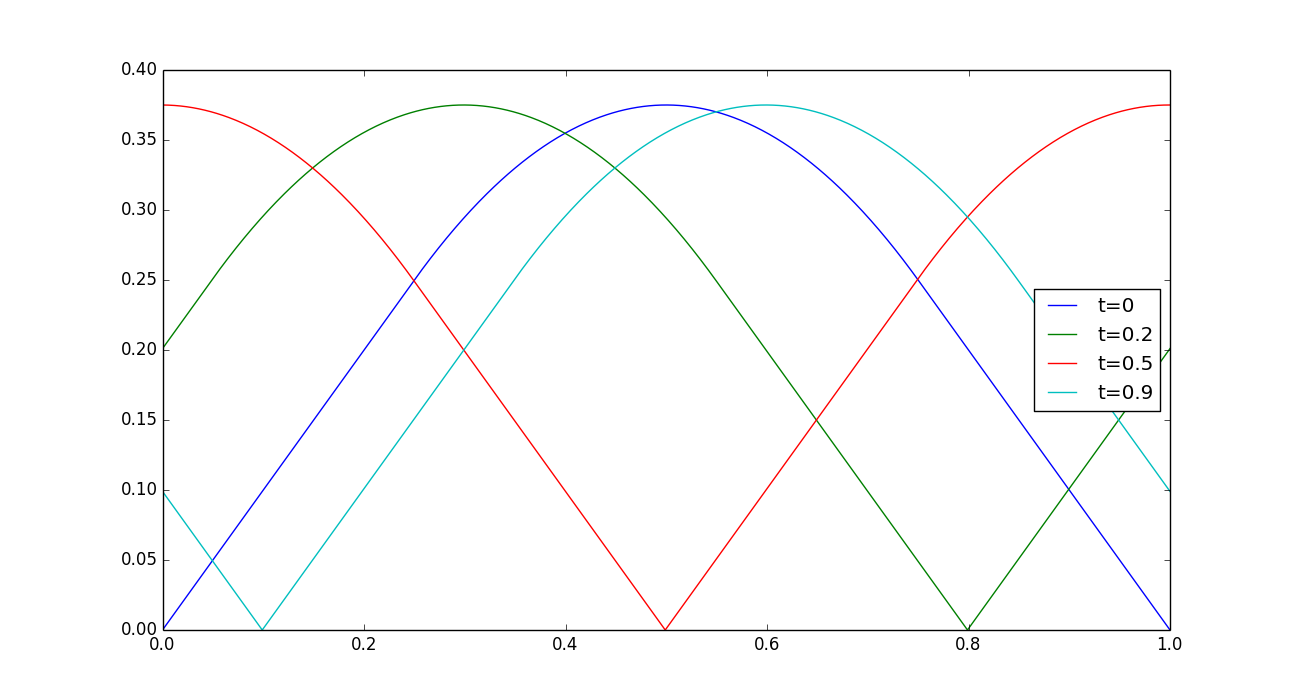
\includegraphics[width = \textwidth]{3_2.png}
  \caption{$u_2(t,x)$, начальные условия №3}
\end{minipage}
\end{figure}




\end{document}
